% !TEX program = xelatex

\documentclass{beamer}
\usepackage[utf8]{inputenc}
\usepackage{listings}
\usepackage{fontspec} % 定制字体
\usepackage{xeCJK}
\usepackage{utopia} %font utopia imported
%\usepackage[UTF8,noindent]{ctexcap}
\usepackage{latexsym,amssymb,amsmath,amsbsy,amsopn,amstext,xcolor,multicol}
\usepackage{graphicx,wrapfig,fancybox}
\usepackage{booktabs}
% \usetheme{Rochester}
\usetheme{Madrid}
\usecolortheme{default}
 % 衬线字体:Linux Libertine
    % BoldFont 可以选择 Bold 字重或者 Semibold 字重
    % BoldItalicFont 也有对应 BoldFont 的字重选择
    % 这里使用 Semibold 字重
    \setmainfont{LinLibertine_R.otf}[
      BoldFont = LinLibertine_RZ.otf,
      ItalicFont = LinLibertine_RI.otf,
      BoldItalicFont = LinLibertine_RZI.otf]
  % % 无衬线字体:Linux Biolinum
  % \setsansfont{LinBiolinum_R.otf}
      %   [BoldFont = LinBiolinum_RB.otf,
      % ItalicFont = LinBiolinum_RI.otf,
      % BoldItalicFont = LinBiolinum_RBO.otf]
  % % 等宽/打印机字体:Linux Libertine Mono
  % \setmonofont{LinLibertine_M.otf}[
  %     BoldFont = LinLibertine_MB.otf,
  %     ItalicFont = LinLibertine_MO.otf,
  %     BoldItalicFont  = LinLibertine_MBO.otf]
  % \setCJKmainfont[ItalicFont={AR PL UKai CN},
  % BoldFont={WenQuanYi Micro Hei}]{IPAMinCho,IPA明朝}
  
  % \setsansfont{Helvetica}
  \setCJKsansfont{WenQuanYi Micro Hei}
  \setCJKmonofont{WenQuanYi Micro Hei Mono}

  \newfontfamily\menlo{WenQuanYi Micro Hei Mono}
  \usepackage{xcolor} % 定制颜色
  \definecolor{mygreen}{rgb}{0,0.6,0}
  \definecolor{mygray}{rgb}{0.5,0.5,0.5}
  \definecolor{mymauve}{rgb}{0.58,0,0.82}
  \lstset{ %
  backgroundcolor=\color{white},      % choose the background color
  basicstyle=\footnotesize\ttfamily,  % size of fonts used for the code
  columns=fullflexible,
  tabsize=4,
  breaklines=true,               % automatic line breaking only at whitespace
  captionpos=b,                  % sets the caption-position to bottom
  commentstyle=\color{mygreen},  % comment style
  escapeinside={\%*}{*)},        % if you want to add LaTeX within your code
  keywordstyle=\color{blue},     % keyword style
  stringstyle=\color{mymauve}\ttfamily,  % string literal style
  frame=single,
  rulesepcolor=\color{red!20!green!20!blue!20},
  % identifierstyle=\color{red},
  language=c++,
  }
  \renewcommand{\thefootnote}{\fnsymbol{footnote}} %*, **, ***
  % \let\thefootnote\relax\footnotetext{Footnotetext without footnote mark}
  %------------------------------------------------------------
%This block of code defines the information to appear in the
%Title page
\title[毕设答辩] %optional
{基于解析数据的DNS安全评估与增强}
\subtitle{毕设答辩}


\author[芦迪] % (optional)
{无41 芦迪}

\institute[THU, EE] % (optional)
{
  \normalsize{指导老师:李星} \\
  \
  
  Department of Electronic Engineering,\\
  Tsinghua University
  
}

\date[2018.6.15] % (optional)
{June 15, 2018}

\logo{
\includegraphics[height=1.5cm]{images/thuee-logo.png}}

%End of title page configuration block
%------------------------------------------------------------



%------------------------------------------------------------
%The next block of commands puts the table of contents at the 
%beginning of each section and highlights the current section:

\AtBeginSection[]
{
  \begin{frame}
    \frametitle{目录}
    \tableofcontents[currentsection]
  \end{frame}
}
%------------------------------------------------------------


\begin{document}
%The next statement creates the title page.
\frame{\titlepage}


%---------------------------------------------------------
%This block of code is for the table of contents after
%the title page
\begin{frame}
\frametitle{目录}
\tableofcontents
\end{frame}
%---------------------------------------------------------
\section{背景介绍}
\begin{frame}{DNS}
  \textbf{DNS}: Domain Name System,域名系统
  \begin{itemize}
    \item 域名(www.tsinghua.edu.cn) \(\Longleftrightarrow\) IP地址(166.111.4.100)
    \item 重要的互联网基础设施,遭到攻击损失无法估量
    \begin{figure}
      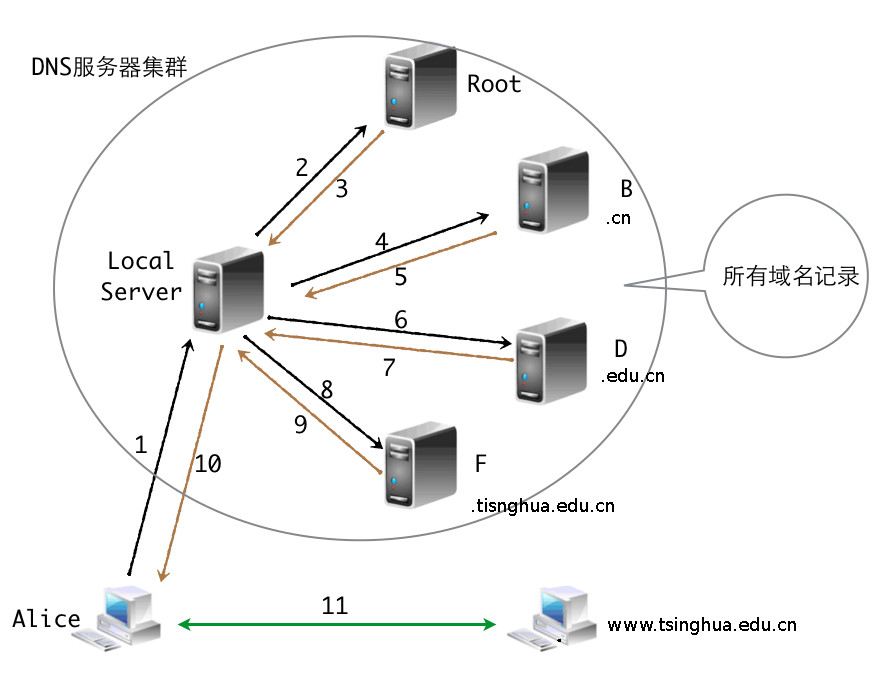
\includegraphics[height=3cm]{figures/dns/name_resolution.jpg}
      \end{figure}
    \item DNS 易受攻击
      \begin{itemize}
        \item  协议脆弱性:UDP、明文;系统脆弱性:Open Resolvers、路径复杂
        \item DNS 劫持:将DNS请求定向到非法解析器
        \item DNS 缓存中毒:将虚假域名数据注入到缓存中
      \end{itemize}
   
  \end{itemize}
  
\end{frame}

\begin{frame}{CDN与负载均衡}
  \begin{itemize}
    \item 因为CDN与负载均衡的普遍存在,域名解析情况更加复杂
    \begin{itemize}
    \item CDN:Content Delivery Network
    \begin{itemize}
      \item 部署边缘服务器,使用户就近获取所需内容,降低网络拥塞
    \end{itemize}
    \begin{figure}
    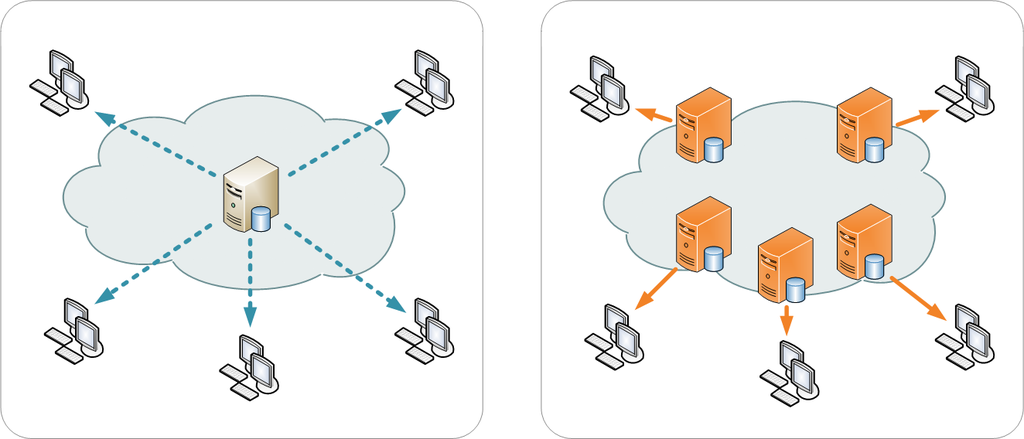
\includegraphics[height=3cm,width=7.07cm]{images/NCDNCDN.png}
    \end{figure}
    
    \item 负载均衡:在多个服务器中分配负载,最优化资源使用,避免过载
    \end{itemize}
    \item 一个域名会解析出多个IP,一个IP也可以对应多个域名
  \end{itemize}

\end{frame}
\begin{frame}{网络安全增强}
  互联网天然缺乏安全性,通过完善协议可以增强安全性
  \begin{itemize}
    \item DNSSEC:DNS安全扩展
    \begin{itemize}
      \item 使用公钥密码机制,以DNS资源记录计算数字签名,验证数字签名确保解析结果真实
      \item 提供数据来源、数据完整性和否定存在验证
    \end{itemize}
    \item IPv6:下一代互联网协议
    \begin{itemize}
      \item IPv6内嵌IPSec协议族的AH和ESP,从协议上提升安全性
      \item IPv6地址空间大,增大扫描难度,可减缓现有攻击
    \end{itemize}
    \item DNS over HTTPS
    \begin{itemize}
      \item 使用HTTPS传输解析信息,增强了客户端和递归解析器之间的隐私和安全性
    \end{itemize}
  \end{itemize}  
\end{frame}

\begin{frame}{毕设内容}
  \begin{itemize}
    \item 分析域名解析数据,了解域名或解析器对IPv6、DNSSEC、HTTPS的支持情况,评估安全现状
    \begin{itemize}
      \item 根据A记录与AAAA记录,判断IPv6支持情况  
      \item 根据RRSIG记录,判断DNSSEC支持情况
      \item 测试(域名, IP地址),判断HTTPS支持情况
    \end{itemize}
    \item 对DNS解析返回的IP地址进行判别与分类
    \begin{itemize}
      \item 结果正常:CDN?负载均衡?
      \item 结果有误:DNS劫持?缓存中毒?
    \end{itemize}
  \end{itemize}
\end{frame}


\begin{frame}{前人工作}
  \begin{itemize}
    \item 文献\cite{Pearce2017}\footnote[1]{Global Measurement of DNS Manipulation}采用一致性和独立的可验证性指标,通过对解析结果IP地址、自治域、HTTP内容、HTTPS证书等内容进行验证,实现了对DNS操作的检测
    \begin{figure}
      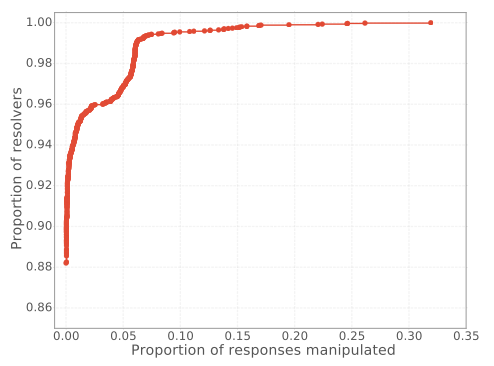
\includegraphics[width=5cm]{images/dnsmanipulate.png}
      \end{figure}
    \item 文献 \cite{Kuhrer}\footnote[7]{Going Wild: Large-Scale Classification of Open DNS Resolvers} 通过对DNS解析结果进行过滤,并对HTTP请求返回的内容进行聚类,系统地分析了非合法的DNS响应
  \end{itemize}
\end{frame}

\section{系统设计}


\section{实验实施}


%---------------------------------------------------------
%Changing visivility of the text
  \begin{frame}{数据获取}
    \begin{columns}
      
      \begin{column}{0.5\textwidth}
        \begin{table}
          \tiny
        \begin{tabular}{r|l|l}
          \toprule
          Resolver& Owner&DNSSEC\\
          \midrule
          8.8.8.8 & Google&Y \\
          4.2.2.2&     MicroSoft&Y \\
          9.9.9.9&  IBM&Y \\
          8.26.56.26& Comodo&Y \\
          180.76.76.76&Baidu&Y\\
          202.141.162.123&USTC&Y\\
          223.6.6.6&Ali&N \\
          114.114.114.114 & 114DNS&N \\
          ......&...... &......\\
          \bottomrule
          \end{tabular}
          \caption{\scriptsize{Open Resolvers}}
        \end{table}
      \end{column}
      \begin{column}{0.5\textwidth}
        \begin{table}
          \tiny
        \begin{tabular}{r|l}
          \toprule
          Num. & Domain Name\\
          \midrule
          1&google.com\\
          2&youtube.com\\
          3&facebook.com\\
          4&baidu.com\\
          5&wikipedia.org\\
          6&yahoo.com\\
          7&reddit.com\\
          8&google.co.in\\
          ......&...... \\
          \bottomrule
          \end{tabular}
          \caption{\scriptsize{Top Domain Names}}
        \end{table}
      \end{column}
      \end{columns}


解析数据获取说明:
  \begin{itemize}
    \item 开放解析器与域名
    \item 工具:MySQL, dnspython
    \item 方式:UDP/TCP, IPv4/IPv6
    \item 腾讯云CVM,公网IP:211.159.174.23
    \item 解析数据的快速获取;频繁请求解析器可能拒绝服务
  \end{itemize}
  \end{frame}
\begin{frame}{数据获取}
  数据库中的IPv4记录与IPv6记录:
  \begin{figure}
    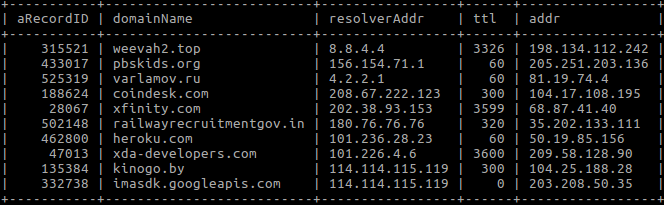
\includegraphics[height=3cm]{images/ipv4sjk.png}
    \end{figure}
    \begin{figure}
      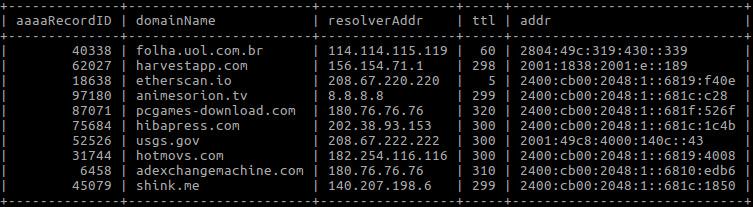
\includegraphics[height=3cm]{images/ipv6sjk.png}
      \end{figure}
\end{frame}
\begin{frame}{数据获取}

  顶级域名分布情况及域名对 IPv6、DNSSEC的支持情况:

  \begin{figure}[htbp]
    \centering
    \begin{minipage}[htbp]{150pt}
      \centering
      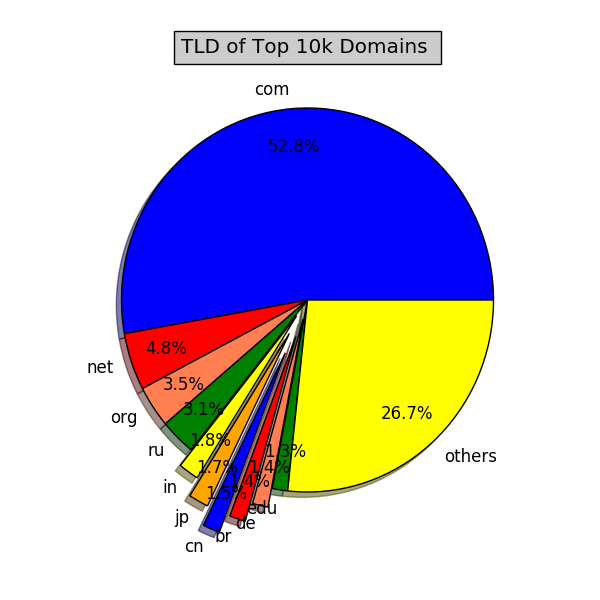
\includegraphics[width=150pt]{images/figure/figure_2.png}
      \caption{\scriptsize{顶级域名分布}}
      \label{fig:4}
    \end{minipage}
    \hspace{10pt}%
    \begin{minipage}[htpb]{150pt}
      \centering
      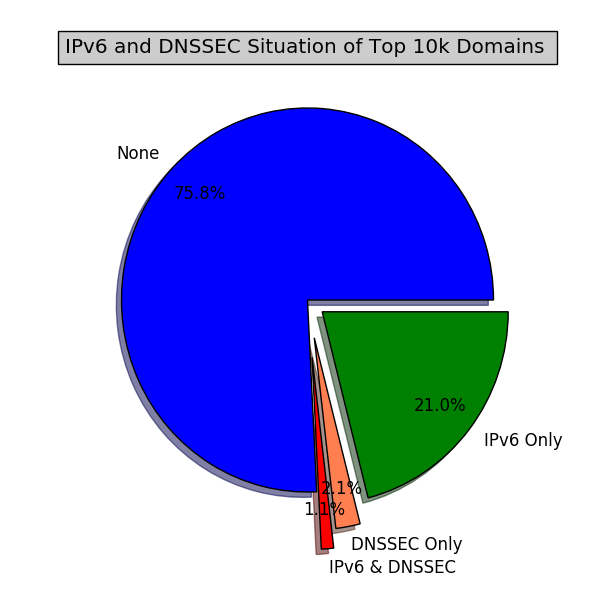
\includegraphics[width=150pt]{images/figure/figure_3.png}
      \caption{\scriptsize{IPv6/DNSSEC Crosscheck}}
      \label{fig:5}
    \end{minipage}
    \end{figure}

% \begin{figure}
%   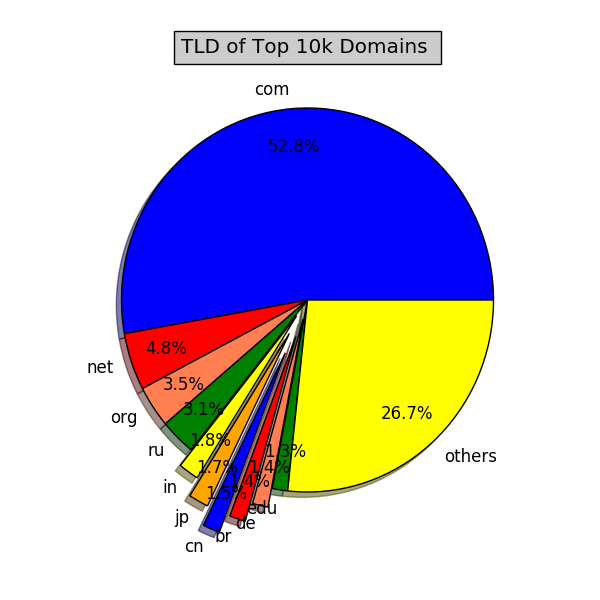
\includegraphics[height=8cm,width=8cm]{images/figure/figure_2.png}
% \end{figure}

\end{frame}
\begin{frame}{数据获取}

  顶级域名.com和.net对 IPv6、DNSSEC的支持情况:

  \begin{figure}[htbp]
    \centering
    \begin{minipage}[htbp]{150pt}
      \centering
      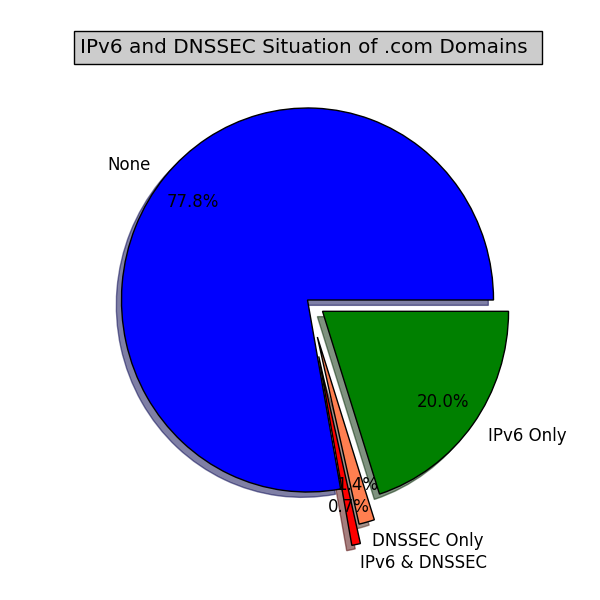
\includegraphics[width=150pt]{images/figure/figure_1.png}
      \caption{\scriptsize{IPv6/DNSSEC Crosscheck in .com Domain}}
      \label{fig:4}
    \end{minipage}
    \hspace{10pt}%
    \begin{minipage}[htpb]{150pt}
      \centering
      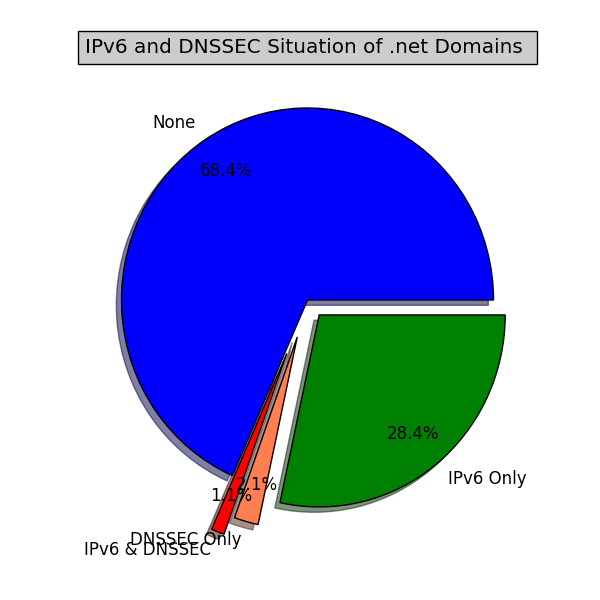
\includegraphics[width=150pt]{images/figure/figure_4.png}
      \caption{\scriptsize{IPv6/DNSSEC Crosscheck in .net Domain}}
      \label{fig:5}
    \end{minipage}
    \end{figure}

% \begin{figure}
%   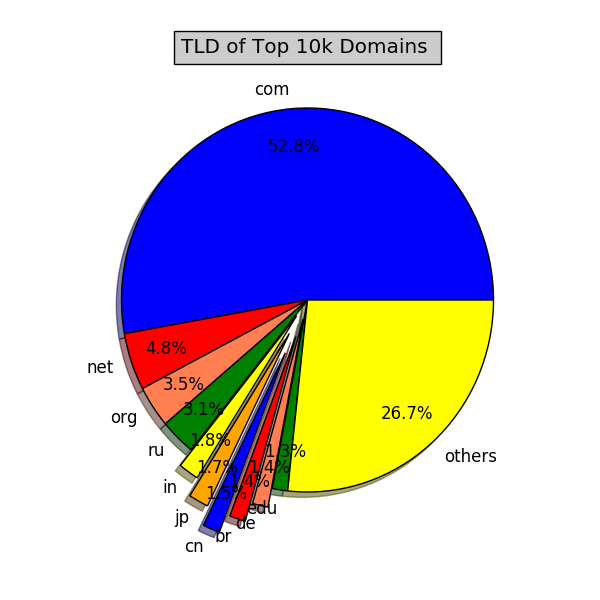
\includegraphics[height=8cm,width=8cm]{images/figure/figure_2.png}
% \end{figure}

\end{frame}

  \begin{frame}{结果标记}
    \begin{itemize}
      \item HTTPS
      \begin{itemize}
        \item 使用数字证书来验证站点的身份,加密用户和站点之间的数据交换
        \item 对于解析到的IP地址,对其 443 端口发起连接请求,验证是否支持HTTPS
        \item 对于支持HTTPS的IP地址,对其证书进行验证,将验证通过的(domain, ip, resolver)对标记为正确
      \end{itemize}
      \item DNSSEC
      \begin{itemize}
        \item 使用数字签名来验证 DNS 数据的完整性,从而确保用户可以到达预期的 IP 地址
        \item 大多数解析器支持 DNSSEC,但部署了 DNSSEC 的域名仍较少
        \item 通过公钥与签名验证解析记录真实性与完整性,从信任锚开始对信任链进行验证
      \end{itemize}
    \end{itemize}
    % \begin{itemize}
    %   \item 所有 Resolver 返回结果相同,说明正常
    %   \item 一些 CDN 解析的结果包含有CNAME记录
    %   % \item 只有负载均衡情况下,服务器IP数量有限
    %   \item 关于DNS劫持的检测,文献\cite{Yan2006}提出了一种基于贝叶斯原理的判别方法
    %   \item 文献\cite{Antonakakis2011}提出了一种名为Kopis的新型检测系统,用于通过被动监控DNS层次结构上层的DNS流量来检测与恶意软件相关的域名
    % \end{itemize}

  \end{frame}

  \begin{frame}{HTTPS结果}
    HTTPS 测试整体情况:
    \begin{columns}
      \begin{column}{0.5\textwidth}
        \begin{table}
          \tiny
        \begin{tabular}{r|l|l|l|l}
          \toprule
                  & Total & Succeeded & Failed &  Refused \\
          \midrule
          (domain, ip) & 47877& 25740 & 1245 &1028\\
          domain name&   8585&5376& 755 &753\\
          \bottomrule
          \end{tabular}
        \end{table}
      \end{column}
      \begin{column}{0.5\textwidth}
        \begin{figure}
          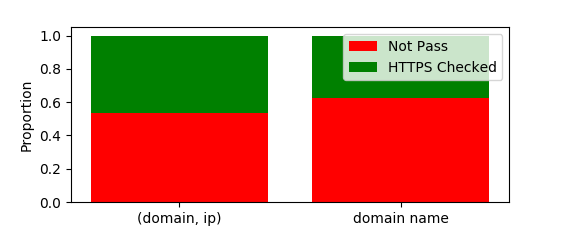
\includegraphics[height=2cm]{images/figure/figure_httpscheck.png}
          \end{figure}
      \end{column}
      \end{columns}
HTTPS 证书服务商统计:
\begin{columns}
      
  \begin{column}{0.5\textwidth}
    \begin{table}
      \tiny
    \begin{tabular}{r|l|l}
      \toprule
      Service Provider &Quantity & Percent\\
      \midrule
      COMODO CA Limited&2006 & 37.22\%\\
      DigiCert Inc&1041& 19.31\%\\
      GlobalSign &393& 7.29\%\\
      GoDaddy.com, Inc.&334& 6.19\%\\
      GeoTrust Inc.&281& 5.21\%\\
      Symantec Corporation&197& 3.65\%\\
      Amazon&190& 3.53\%\\
      CloudFlare, Inc.&157& 2.91\%\\
      Google Trust Services&148& 2.75\%\\
      Others & 643& 11.93\%\\
      \bottomrule
      \end{tabular}
    \end{table}

  \end{column}
  \begin{column}{0.5\textwidth}
    \begin{figure}
      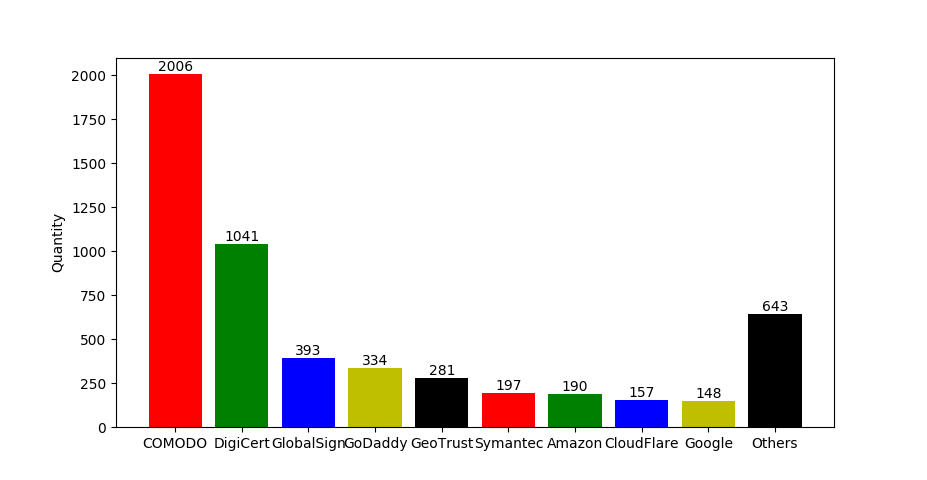
\includegraphics[height=3.5cm]{images/figure/certserver.png}
      \end{figure}
  \end{column}
  \end{columns}



    
  \end{frame}
\section{数据分析}
  \begin{frame}{HTTPS/DNSSEC分析}

  \begin{figure}
    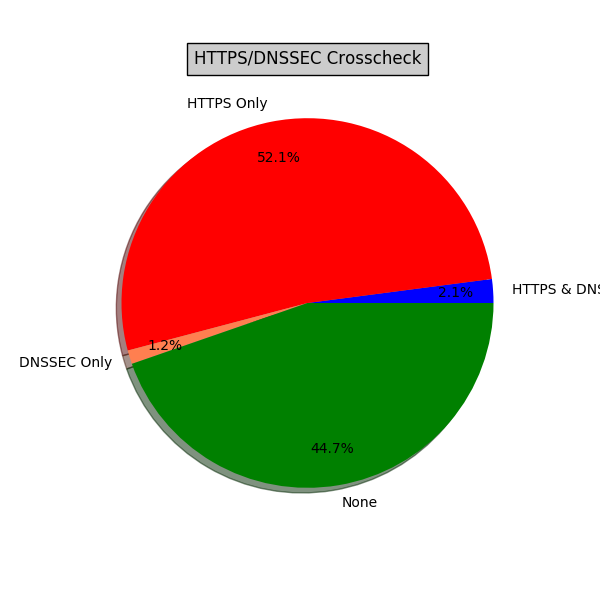
\includegraphics[height=5cm,width=5cm]{images/figure/httpsdnssec.png}
  \end{figure}
  对于 DNSEC Only 的情况,发现以以下三类网站居多:
  \begin{itemize}
    \item 成人网站
    \item 教育机构
    \item 政府机构
  \end{itemize}
  \end{frame}
  

  \begin{frame}{HTTPS/DNSSEC分析}
  对顶级域名 .com 和 .net 对DNSSEC和HTTPS支持情况进行分析:
    \begin{figure}[htbp]
      \centering
      \begin{minipage}[htbp]{150pt}
        \centering
        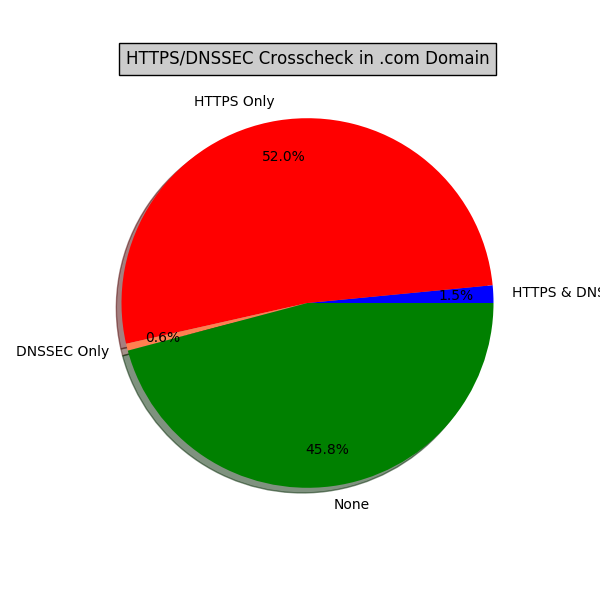
\includegraphics[width=150pt]{images/figure/httpsdnsseccom.png}
        \label{fig:4}
      \end{minipage}
      \hspace{10pt}%
      \begin{minipage}[htpb]{150pt}
        \centering
        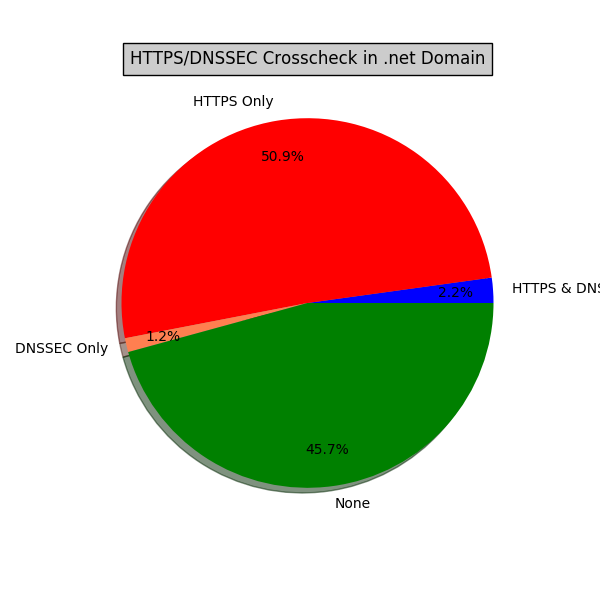
\includegraphics[width=150pt]{images/figure/httpsdnssecnet.png}
        \label{fig:5}
      \end{minipage}
      \end{figure}
  
  % \begin{figure}
  %   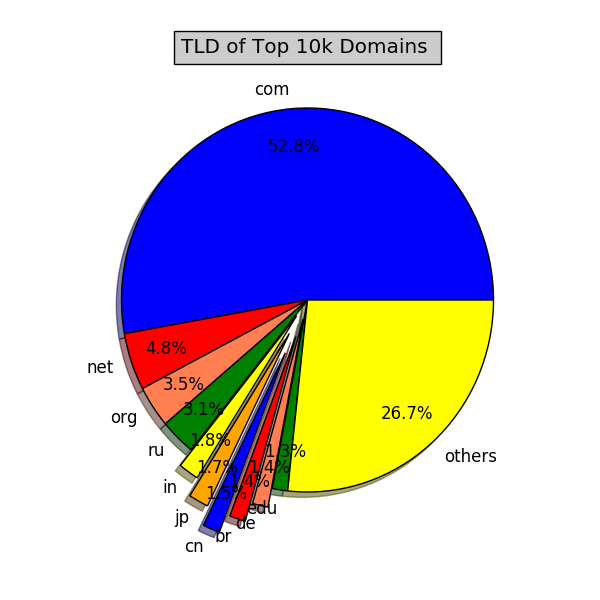
\includegraphics[height=8cm,width=8cm]{images/figure/figure_2.png}
  % \end{figure}
  
  \end{frame}
  \begin{frame}{数据分析}
    对证书中获取的国家名称进行分析:
    \begin{figure}
      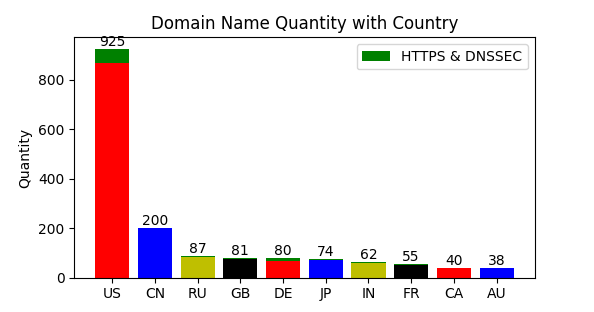
\includegraphics[width=8cm]{images/figure/quantitycountry2.png}
    \end{figure}
  
    \end{frame}
  % \begin{frame}{初步分析}
  % \begin{figure}
  %   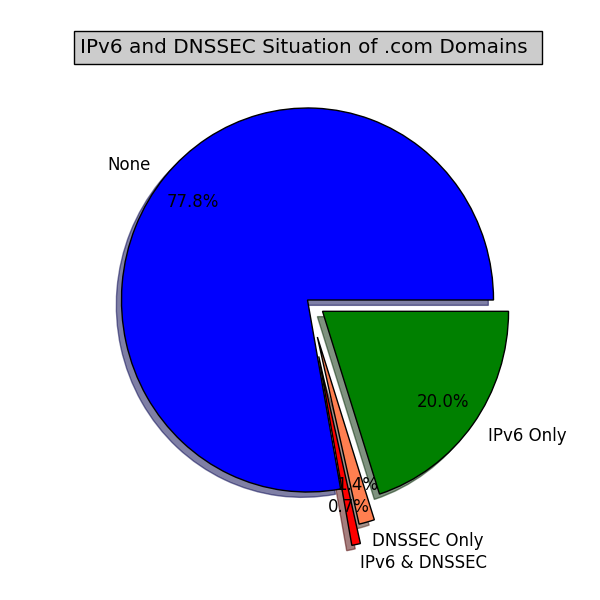
\includegraphics[height=8cm,width=8cm]{images/figure/figure_1.png}
  % \end{figure}
  % \end{frame}
  % \begin{frame}{初步分析}
  % \begin{figure}
  %   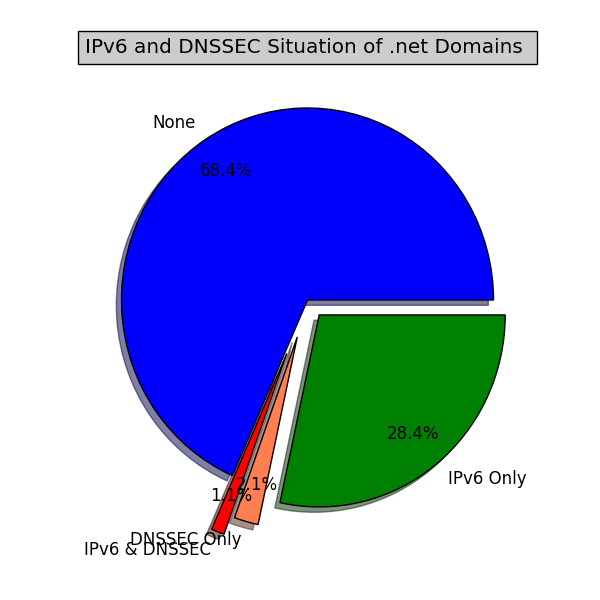
\includegraphics[height=8cm,width=8cm]{images/figure/figure_4.png}
  % \end{figure}

  % \end{frame}




 \begin{frame}{参考文献}
  \tiny
  \bibliographystyle{unsrt}%Used BibTeX style is unsrt
  \bibliography{ref}
\end{frame}

\begin{frame}
  \begin{figure}
    
\includegraphics[height=2.23cm,width=4.29cm]{images/thank.jpg}
  \end{figure} 
\end{frame}
\end{document}

